\section{\texorpdfstring{$p(x) = \sum_{i=0}^{n}\lambda_ix^i$}{p(x) = summe i = 
0 bis n lambdai xi}}
\rhead{$p(x) = \sum_{i=0}^{n}\lambda_ix^i$}

Aufgrund der bisherigen Beobachtungen ist es nun m"oglich, eine 
allgemein geltende Potenzreihenl"osung f"ur diese Art Differentialgleichungen 
zu erstellen. Hierzu wird das anf"angliche parabolische Profil $ax^2 + bx + c$ 
durch das allgemeine Polynomprofil $n$-ten Grades
\begin{equation*}
	p(x) =
	\lambda_nx^n + \lambda_{n-1}x^{n-1} + \lambda_{n-2}x^{n-2} + \dotsb + 
	\lambda_2x^2 + \lambda_1x + \lambda_0 = \sum_{i=0}^{n}\lambda_ix^i, \quad n 
	\ge 0
\end{equation*}
ersetzt.

Bei der neuen Problemstellung handelt es sich immer noch um eine 
Differentialgleichung zweiter Ordnung. Es bleibt also eine Abh"angigkeit von 
mindestens zwei Elementen zwischen den verschiedenen $a_k$. Zus"atzlich erh"oht 
sich diese jeweils um den Index $i$ aufgrund der Verschiebung der $a_k$ nach 
rechts, wie im Abschnitt \ref{subsec:wellen:Potenzreihenansatz} gezeigt wurde. 
Daraus folgt die Rekursionsformel
\index{Rekursionsformel}%
\begin{align}
	a_k &= -\frac{1}{k(k-1)}\sum_{i=0}^{n}a_{k-2-i}\lambda_i, \quad n \ge 0, 
	&a_{k-2-i < 0} &=  0
	\label{eq:wellen:allgemeineak}
\end{align}
f"ur ein Polynom $n$-ten Grades.

\subsubsection{Schlussfolgerungen}

Mit der Formel (\ref{eq:wellen:allgemeineak}) gibt es ein einfaches 
Werkzeug mit dem man, allein durch Einsetzen der Parameter, die Koeffizienten 
der Potenzreihenl"osung f"ur diese Art von Differentialgleichungen erh"alt.

Sie erlaubt es uns zudem auch noch weitere Schl"usse zu ziehen. Man kann direkt 
aus der Form des gegebenen Polynomprofils ablesen, wie sich die 
Differentialgleichung verhalten wird. Soll heissen, positive Werte
f"uhren zu einer Wellenform, die Sinus und Cosinus enthalten, negative 
Werte liefern hingegen eine exponentielle Form aus Sinus Hyperbolicus und 
Cosinus Hyperbolicus.

\subsubsection{Berechnungsaufwand}

Es ergibt sich somit der 
Pseudocode (\ref{alg:wellen:allgemeinepotenzreihenrechnung}) f"ur die 
allgemeine Potenzreihenl"osung dieser Differentialgleichung.

\begin{algorithm}
	\floatname{algorithm}{Pseudocode}
	\begin{algorithmic}[1]
		\State $j \gets 1$
		\For{$j \le n$}
			\State $a_{-j} \gets 0$
		\EndFor
		\State $a_0 \gets y(0)$
		\State $a_1 \gets y'(0)$
		\State $x \gets x_{\text{min}}$
		\For{$x \le x_{\text{max}}$}
			\State $k \gets 2$
			\State $s_{\text{pot}} \gets a_0 + a_1x$
			\For{$k \le k_{\text{max}}$}
				\State $s_{\text{pol}} \gets 0$
				\State $i \gets 0$
				\For{$i \le n$}
					\State $s_{\text{pol}} \gets s_{\text{pol}}+\lambda_i 
					a_{k-2-i}$
					\State $i \gets i + 1$
				\EndFor
				\State $a_k \gets -\cfrac{1}{k(k-1)} s_{\text{pol}}$
				\State $s_{\text{pot}} \gets s_{\text{pot}} + a_k x^k$
				\State $k \gets k + 1$
			\EndFor
			\State $x \gets x + x_{\text{step}}$
		\EndFor
	\end{algorithmic}
	
	\caption{Allgemeine Potenzreihenberechnung} 
	\label{alg:wellen:allgemeinepotenzreihenrechnung}
\end{algorithm}

Der allgemeine Algorithmus mit dem Pseudocode 
(\ref{alg:wellen:allgemeinepotenzreihenrechnung}) hat eine Laufzeit von
\begin{equation*}
	\mathcal{O}
	\left(
		nk_{\text{max}}\frac{x_{\text{max}}-x_{\text{min}}}{x_{\text{step}}}
	\right)
\end{equation*}
und einem Speicherverbrauch von
\begin{equation*}
	\mathcal{O}
	\left(
		n
	\right).
\end{equation*}

\begin{algorithm}
	\floatname{algorithm}{Pseudocode}
	\begin{algorithmic}[1]
		\State $j \gets 1$
		\For{$j \le n$}
			\State $a_{-j} \gets 0$
		\EndFor
		\State $a_0 \gets y(0)$
		\State $a_1 \gets y'(0)$
		\State $k \gets 2$
		\For{$k \le k_{\text{max}}$}
			\State $s_{\text{pol}} \gets 0$
			\State $i \gets 0$
			\For{$i \le n$}
				\State $s_{\text{pol}} \gets s_{\text{pol}}+\lambda_i a_{k-2-i}$
				\State $i \gets i + 1$
			\EndFor
			\State $a_k \gets -\cfrac{1}{k(k-1)} s_{\text{pol}}$
			\State $k \gets k + 1$
		\EndFor
		\State $x \gets x_{\text{min}}$
		\For{$x \le x_{\text{max}}$}
			\State $s_{\text{pot}} \gets a_0 + a_1x$
			\State $k \gets 2$
			\For{$k \le k_{\text{max}}$}
				\State $s_{\text{pot}} \gets s_{\text{pot}} + a_k x^k$
				\State $k \gets k + 1$
			\EndFor
			\State $x \gets x + x_{\text{step}}$
		\EndFor
	\end{algorithmic}
	\caption{Allgemeine Potenzreihenberechnung (Alternative)} 
	\label{alg:wellen:allgemeinepotenzreihenrechnungalt}
\end{algorithm}

Alternativ kann man auch Pseudocode 
\ref{alg:wellen:allgemeinepotenzreihenrechnungalt} verwenden. Dieser hat eine 
Laufzeit von
\begin{equation*}
	\mathcal{O}
	\left(
		nk_{\text{max}} + k_{\text{max}} 
		\frac{x_{\text{max}}-x_{\text{min}}}{x_{\text{step}}}
	\right)
	=
	\mathcal{O}
	\left(
		k_{\text{max}}
		\left(
			n+\frac{x_{\text{max}}-x_{\text{min}}}{x_{\text{step}}}
		\right)
	\right),
\end{equation*}
mit einem Speicherverbrauch von
\begin{equation*}
	\mathcal{O}
	\left(
		\max(n, k_{\text{max}})
	\right).
\end{equation*}

Eine Implementation mit \texttt{octave} hat gezeigt dieser alternative 
Algorithmus (Pseudocode \ref{alg:wellen:allgemeinepotenzreihenrechnungalt}) 
fast 10-Mal schneller ist. Dies liegt neben der zus"atzlichen inneren Schlaufe 
auch vor allem daran, dass beim anderen Algorithmus mit \texttt{modulo} 
gerechnet werden musste um den Speicherverbrauch zu optimieren, was 
zus"atzlichen Rechenaufwand bedeutet.

\subsection{\texorpdfstring{$y''-xy = 0$}{y''-xy = 0}}
Die Koeffizienten der uns bereits bekannten Airy-Differentialgleichung k"onne 
durch einfaches Einsetzen in die Formel (\ref{eq:wellen:allgemeineak}) 
berechnet werden.

\begin{equation*}
	\begin{split}
		a_k &= -\frac{1}{k(k-1)} ((-1) a_{k-2-1} + 
		0 a_{k-2-0})
		\\
		&= \frac{1}{k(k-1)} a_{k-3}, \qquad a_{k < 0} = 0,
	\end{split}
\end{equation*}
was sich mit den bereits bekannten L"osung deckt.

Auch die genannten Konsequenzen werden in der Abbildung 
\ref{fig:wellen:airy-dgl} deutlich aufgezeigt.

\begin{figure}
	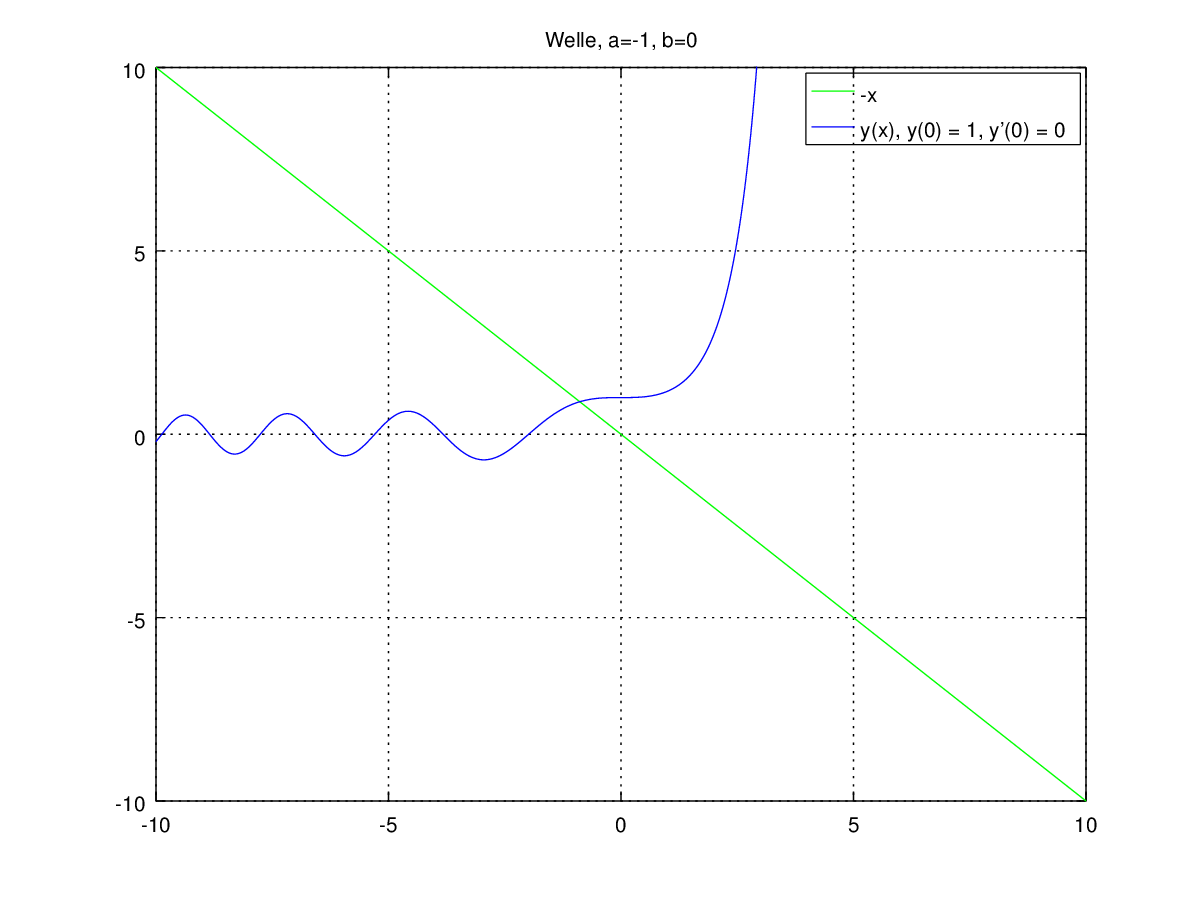
\includegraphics[scale=0.65]{./wellen/images/allgemein/n1.png}
	\caption{L"osung Airy-Differentialgleichung}
	\label{fig:wellen:airy-dgl}
\end{figure}

\subsection{\texorpdfstring{$y''+(ax^4+bx^3+cx^2+dx+e)y = 
0$}{y''-(ax4+bx3+cx2+dx+e)y = 0}}

Auch ein Polynom 4-ten Grades stellt kein Problem mehr dar. Die 
Differentialgleichung:

\begin{equation*}
	y''+(ax^4+bx^3+cx^2+dx+e)y = 0
\end{equation*}
ergibt nach dem Einsetzen:

\begin{align*}
	y(x) &= a_0+a_1x-\sum_{k=2}^{\infty} \frac{1}{k(k-1)} (aa_{k-2-4} + 
	ba_{k-2-3} + ca_{k-2-2} + da_{k-2-1} +ea_{k-2-0})x^k
	\\
	&= a_0+a_1x-\sum_{k=2}^{\infty} \frac{1}{k(k-1)} (aa_{k-6} + ba_{k-5} + 
	ca_{k-4} + da_{k-3} +ea_{k-2})x^k, \qquad a_{k<0} = 0
\end{align*}

Auch hier können wir in der Abbildung (\ref{fig:wellen:poly4-dgl}) die 
"Uberg"ange zwischen $\sin$ und $\cos$ bei positiven und $\sinh$ und $\cosh$ 
bei negativen Polynoml"osungen klar erkennen.

\begin{figure}
	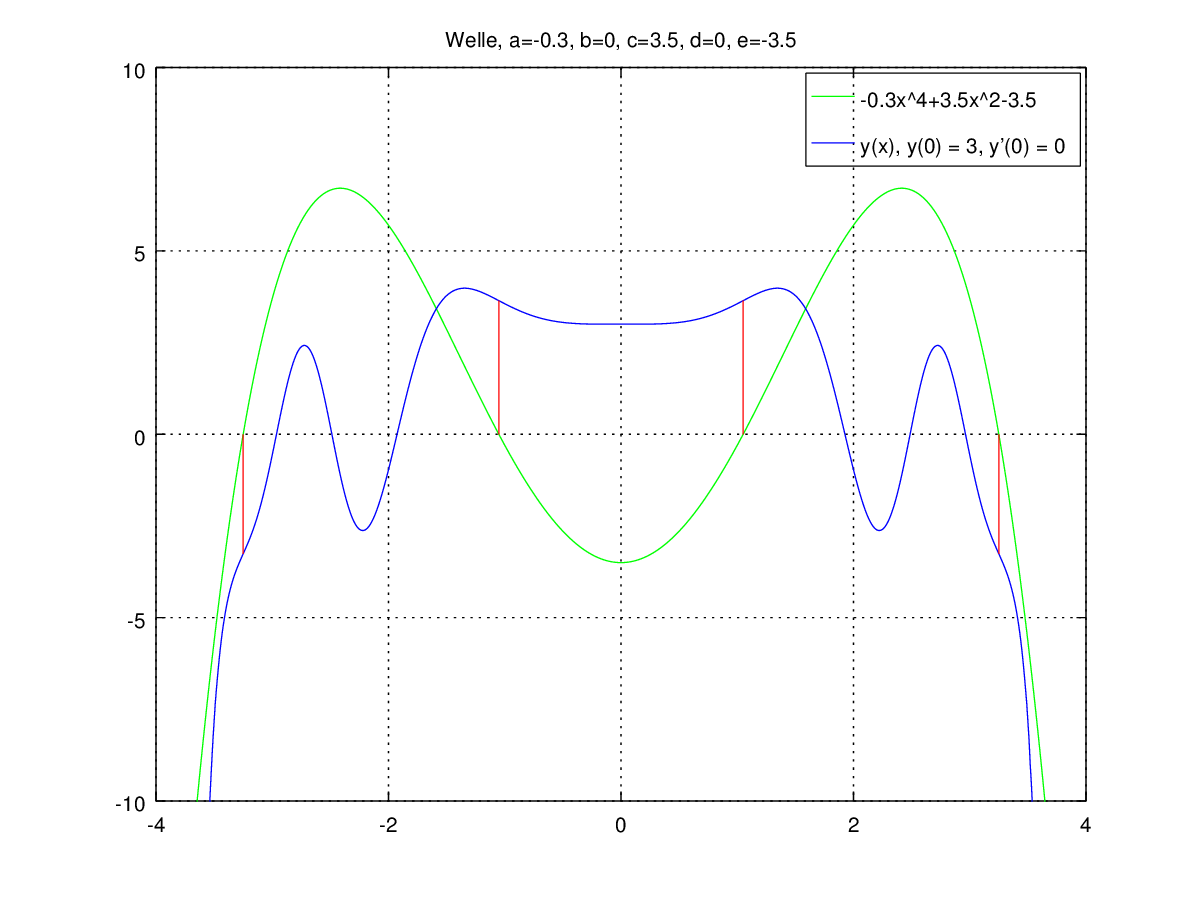
\includegraphics[scale=0.65]{./wellen/images/allgemein/n4.png}
	\caption{L"osung Polynom 4-ten Grades}
	\label{fig:wellen:poly4-dgl}
\end{figure}
